%! suppress = Makeatletter
%! suppress = TooLargeSection
%! suppress = MissingLabel
\documentclass{article}

% Fields
\usepackage{geometry}
\geometry{top=25mm}
\geometry{bottom=35mm}
\geometry{left=20mm}
\geometry{right=20mm}
% ------------------------------------------------

% Graphics
\usepackage{color}
\usepackage{tabularx}
\usepackage{tikz}
\usepackage{blkarray}
\usepackage{graphicx}
% ------------------------------------------------

% Math
\usepackage{amsmath, amsfonts}
\usepackage{amssymb}
\usepackage{proof}
\usepackage{mathrsfs}
% Crossed-out symbols
% https://tex.stackexchange.com/questions/75525/how-to-write-crossed-out-math-in-latex
\usepackage[makeroom]{cancel}
\usepackage{mathtools}
% ------------------------------------------------

% Additional font sizes
% https://www.overleaf.com/learn/latex/Questions/How_do_I_adjust_the_font_size%3F
\usepackage{moresize}
% Additional colors
% https://www.overleaf.com/learn/latex/Using_colours_in_LaTeX
\usepackage{xcolor}
% \texttimes
\usepackage{textcomp}
% ------------------------------------------------

% Language
\usepackage[utf8] {inputenc}
\usepackage[T2A] {fontenc}
\usepackage[english, russian] {babel}
\usepackage{indentfirst, verbatim}
\usetikzlibrary{cd, babel}
% ------------------------------------------------

% Fonts
\usepackage{stmaryrd}
\usepackage{cmbright}
\usepackage{wasysym}
% ------------------------------------------------

% Code
% https://tex.stackexchange.com/questions/99475/how-to-invoke-latex-with-the-shell-escape-flag-in-texstudio-former-texmakerx
% Colored, requires --shell-escape compiling option
% \usepackage{minted}
% \setminted{xleftmargin=\parindent, autogobble, escapeinside=\#\#}
\usepackage{listings}
% ------------------------------------------------

% Custom envs
% https://tex.stackexchange.com/questions/371286/draw-a-horizontal-line-in-latex
\newenvironment{proof}{\subparagraph{\hspace{-1em}Решение:\newline}}{\par\noindent\rule{\textwidth}{0.4pt}}
% ------------------------------------------------

% Custom commands
\newcommand{\comb}[1]{\mathbf{#1}}
\newcommand{\step}{\rightsquigarrow}
\newcommand{\term}[1]{\mathbf{#1}}
\newcommand{\ap}{~}
\newcommand{\termdef}{\coloneqq}
\newcommand{\subst}[3]{\left[#2 \mapsto #3 \right] #1}
\newcommand{\eqbeta}{=_\beta}
\newcommand{\eqeta}{=_\eta}
\def\multiset#1#2{\ensuremath{\left(\kern-.3em\left(\genfrac{}{}{0pt}{}{#1}{#2}\right)\kern-.3em\right)}}
% ------------------------------------------------

% Head
\usepackage{fancybox,fancyhdr}
\usepackage{hyperref}
\pagestyle{fancy}
\fancyhead[R]{Максим Васильев (285800)} % TODO введите ваше имя
\fancyhead[L]{ИТМО MSE, ДМ 2023, Дз 12}
% ------------------------------------------------

% Numbering
% https://tex.stackexchange.com/questions/80113/hide-section-numbers-but-keep-numbering
\makeatletter
\renewcommand\thesubsection{Блок \@arabic\c@subsection.\hspace{-0.8em}}
\renewcommand\thesubsubsection{Задание \@arabic\c@subsection.\@arabic\c@subsubsection\hspace{-0.8em}}
% https://tex.stackexchange.com/questions/327689/numbering-subsubsections-with-letters
\renewcommand\theparagraph{\alph{paragraph})\hspace{-0.8em}}
% https://tex.stackexchange.com/questions/129208/numbering-paragraphs-in-latex
\setcounter{secnumdepth}{4}
\makeatother
% ------------------------------------------------

\begin{document}
\begin{enumerate}
    \item \textit{(0,5 балла)} Докажите, что любое дерево является двудольным графом.
    
    \textbf{Решение}:

    Граф называется двудольным, если множество его вершин можно разбить на два непересекающихся подмножества таким образом, чтобы никакие две вершины из одного множества не были соединены ребром.

    Деревом называется простой связных граф, в котором между любыми двумя вершинами существует единственный путь.

    Покажем, что множество вершин дерева всегда можно разбить на два множества так, чтобы получился двудольный граф. Для этого зафиксируем какую-нибудь вершину дерева $v$ и отнесем ее к первому множеству. Дальше будем перебирать все вершины по порядку, и если длина пути до очередной вершины нечетна, то будем относить ее ко второму множеству, а если четна, то к первому. В итоге получим два непересекающихся множества вершин, объединение которых даст исходное множество вершин графа.

    Покажем, что любые две вершины $v_1, v_2$, обладающие одним ребром, лежат в разных подмножествах. Для этого возьмем какую-нибудь вершину $v'$ из первого множества и предположим, что вершина $v_1$ тоже лежит в первом множестве. Так как они лежат в одном подмножестве вершин, то путь от одной до другой - четный. Так как путь между любыми двумя вершинами в дереве единственный, то путь между $v'$ и $v_2$ обязательно проходит по ребру $v_1, v_2$, поэтому путь от $v'$ до $v_2$ нечетный, поэтому вершины $v_1, v_2$ лежат в разных подмножествах. $\blacksquare$

    \item \textit{(1 балл)} Полным $m$-арным деревом называется корневое дерево, у которого любая вершина, отличная от листа, имеет ровно $m$ сыновей. Предположим, что у такого дерева имеется k вершин, отличных от листа. Найдите количество листьев в таком дереве.
    
    \textbf{Решение}:

    Обозначим число листьев через $x$. Тогда в дереве всего $k+x$ вершин -- вершины со степенями, отличными от 1 и равными 1. Зная количество вершин, можно определить количество ребер в дереве:
    \begin{equation}
        N = k+x-1.
    \end{equation}
    С другой стороны количество ребер можно посчитать как количество вершин на количество сыновей каждого (так как дерево полное):
    \begin{equation}
        N = m \cdot k.
    \end{equation}
    Отсюда получается выражение:
    \begin{equation}
        k+x-1 = m \cdot k \Rightarrow x = k(m-1)+1.
    \end{equation}
    Тогда количество листьев в полном $m$-арном дереве равно

    \textbf{Ответ}: $k(m-1)+1$.

    \item \textit{(1 балл)} Найдите количество неизоморфных друг другу деревьев на $n \geq 4$ вершинах, диаметр которых меньше или равен трем.
    
    \textbf{Решение}:
    
    Построим конструктивное решение сначала для диаметра, равного 2, а потом для 3 (для меньших диаметров решений не существует, потому что деревья -- связные графы).
    \begin{itemize}
        \item $d = 2$:
        
        Возьмем две вершины и соединим их. Получилась симметричная ситуация, поэтому добавим еще одну вершину, присоединенную к любой из уже существующих. Теперь получается так, что диаметр равен 2, и увеличивать его нельзя, поэтому можно добавлять новые вершины, соединяя из только с изначальными двумя вершинами. В таком случае мы получаем правило, по которому можно строить бесконечное количество неизоморфных деревьев на $n \geq 4$ вершинах с диаметром, равным 2.

        \item $d = 2$:
        
        Возьмем четыре вершины и соединим их последовательно. Получилась симметричная ситуация, в которой диаметр такого дерева равен 3.  Теперь из такой картинки можно получить бесконечное количество неизоморфных деревьев на $n \geq 4$ вершинах с диаметром, равным 3, по следующему правилу: к вершинам под номерами 2 и 3 (из последовательного списка 1, 2, 3, 4) можно присоединять дополнительные листья. При таком построении диаметр не будет никак изменяться, потому что мы добавляем лишь листья, которые находятся наравне с листьями 1 и 4. $\blacksquare$
    \end{itemize}
    
    \item \textit{(1 балл)} Пусть T — дерево, в котором степень любой вершины, смежной с листом, больше или равна трем. Докажите, что в T обязательно найдется пара листьев, имеющих общего соседа.
    
    \textbf{Решение}:
    
    Найдем максимальный путь в дереве T. Выразим его через последовательность вершин (можно сделать, так как T -- дерево): $\{a, b, c, \dots\}$. Так как путь максимальный, то вершина $a$ обязательно должна быть листом, иначе был бы более длинный путь. Так как $a$ -- лист, то степень вершины $b$ больше или равна 3 (по условию). Поэтому у вершины $b$ есть еще одно ребро, которое ведет в другую вершину $d$. Эта вершина $d$ обязана быть листом, потому что в противном случае существовал бы более длинный путь в дереве. Итого, если в дереве T степень любой вершины, смежной с листом, больше или равна 3, то в T обязательно найдется пара листьев, имеющих общего соседа. $\blacksquare$

    \item \textit{(0.5 балла)} Постройте последовательность Прюфера для данного дерева:
    
    \begin{figure}[h]
        \centering
        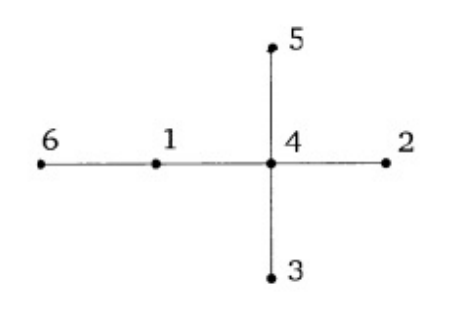
\includegraphics[width=0.35\textwidth]{images/12.5.png}
    \end{figure}

    \textbf{Решение}:
    
    \begin{table}[h]
        \centering
        \begin{tabular}{|c|c|c|c|}
            \hline
            Номер шага & Минимальный лист & Родитель & Последовательность \\
            \hline
            1 & 2 & 4 & \{4\} \\
            \hline
            2 & 3 & 4 & \{4, 4\} \\
            \hline
            3 & 5 & 4 & \{4, 4, 4\} \\
            \hline
            4 & 4 & 1 & \{4, 4, 4, 1\} \\
            \hline
        \end{tabular}
    \end{table}
    
    \textbf{Ответ}: \{4, 4, 4, 1\}.

    \item \textit{(0.5 балла)} Постройте дерево, отвечающее последовательности Прюфера $(1, 7, 2, 2, 2, 2)$.
    
    \textbf{Решение}:
    
    \begin{table}[h]
        \centering
        \begin{tabular}{|c|c|c|c|}
            \hline
            Номер шага & Текущий код Прюфера & Доступные вершины & Ребра \\
            \hline
            1 & 1, 7, 2, 2, 2, 2 & 1, 2, 3, 4, 5, 6, 7, 8 & \\
            \hline
            2 & 7, 2, 2, 2, 2 & 1, 2, 4, 5, 6, 7, 8 & 1-3 \\
            \hline
            3 & 2, 2, 2, 2 & 2, 4, 5, 6, 7, 8 & 1-3, 1-7 \\
            \hline
            4 & 2, 2, 2 & 2, 5, 6, 7, 8 & 1-3, 1-7, 2-4 \\
            \hline
            5 & 2, 2 & 2, 6, 7, 8 & 1-3, 1-7, 2-4, 2-5 \\
            \hline
            6 & 2 & 2, 7, 8 & 1-3, 1-7, 2-4, 2-5, 2-6 \\
            \hline
            7 & & 2, 8 & 1-3, 1-7, 2-4, 2-5, 2-6, 2-7 \\
            \hline
            8 & & & 1-3, 1-7, 2-4, 2-5, 2-6, 2-7, 2-8 \\
            \hline
        \end{tabular}
    \end{table}
    \begin{tikzpicture}
        % Вершины
        \foreach \i/\angle in {1/45, 3/90, 4/135, 5/180, 6/225, 7/270} {
          \node[circle, draw, fill=black, inner sep=2pt, label=above:$\i$] (\i) at (\angle:2) {};
        }
        % Центральная вершина 2
        \node[circle, draw, fill=black, inner sep=2pt, label=above:$2$] (2) at (0,0) {};
        \node[circle, draw, fill=black, inner sep=2pt, label=above:$8$] (8) at (0.7,0.7) {};
        % Рёбра
        \foreach \x/\y in {1/3, 1/7, 2/4, 2/5, 2/6, 2/7, 2/8} {
          \draw (\x) -- (\y);
        }
    \end{tikzpicture}

    % \item \textit{(1.5 балла)} Подсчитайте количество всех деревьев, построенных на множестве вершин $[n]$, у которых вершина с меткой $i$ имеет степень $d_i$. Выведите отсюда формулу Кэли для количества всех деревьев на n вершинах.
\end{enumerate}
\end{document}
